\documentclass[aspectratio=169]{beamer}

\useoutertheme{infolines}

\usepackage{graphicx}
\usepackage{subcaption}

\title{PNLSS Identification}
\subtitle{Post TRC Institute Meeting 3}
\author[Balaji, N. N.]{Nidish Narayanaa Balaji}
\institute[Rice U.]{Rice University, Houston, TX 77005}
\date{October 10, 2019}
\begin{document}
\maketitle{}

\section{Benchmark 1}
\label{sec:benchmark-1}
\begin{frame}  
  \frametitle{Progress on Benchmark 1 (Duffing Oscillator)}
  \framesubtitle{Overview}  
  \begin{itemize}
  \item Conducted PNLSS with different amplitude levels (as before)
  \item Constructed frequency response with PNLSS model
  \item Synthesized frequency response with identified data from
    simulated experiments from Eve (without shaker model)
  \end{itemize}
  \textbf{To Do:}
  \begin{itemize}
  \item Consider shaker model
  \end{itemize}
\end{frame}

\begin{frame}[allowframebreaks]
  \frametitle{Progress on Benchmark 1 (Duffing Oscillator)}
  \framesubtitle{Frequency Response Comparisons}
  \vspace{-0.5cm}
  \hspace{12cm}(Non-periodic)
  \vspace{-0.5cm}
  \begin{figure}
    \centering
    \begin{subfigure}{0.25\linewidth}
      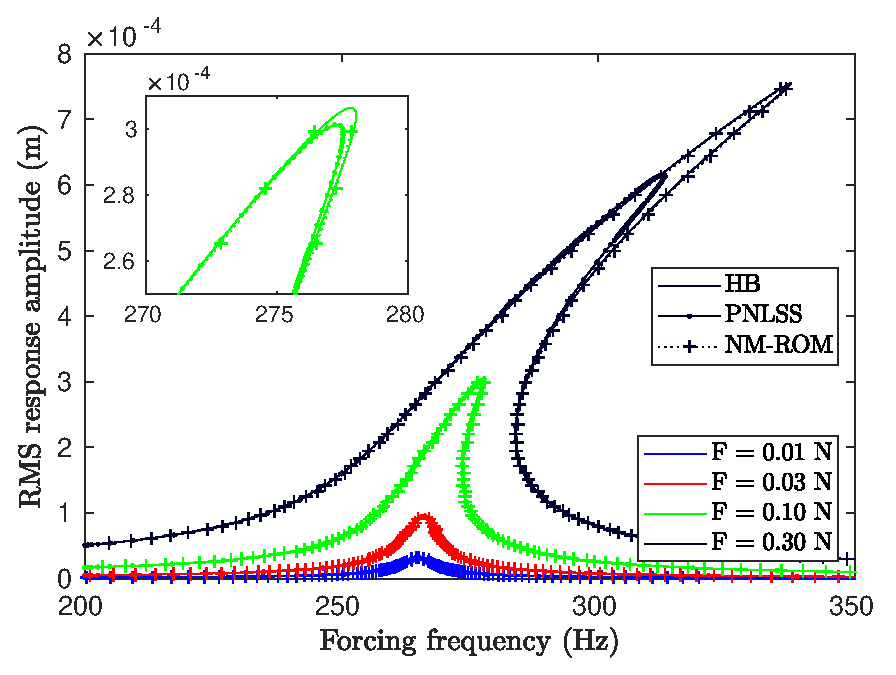
\includegraphics[width=\linewidth]{{{../../benchmark1/extabs_fig/b1_fresp_comp_A0.01_nx23}}}
    \end{subfigure}%
    \begin{subfigure}{0.25\linewidth}
      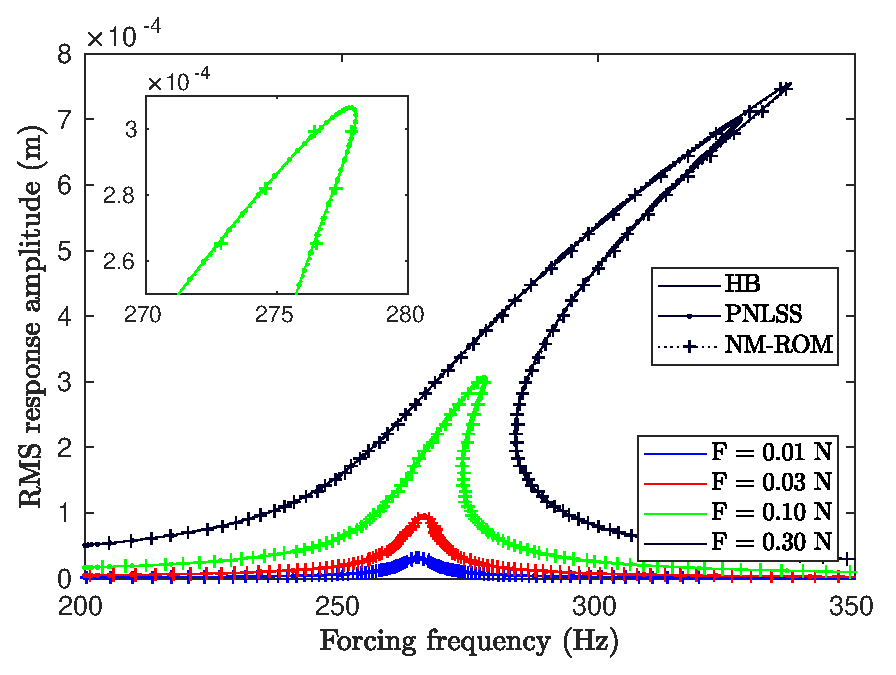
\includegraphics[width=\linewidth]{{{../../benchmark1/extabs_fig/b1_fresp_comp_A0.25_nx23}}}
    \end{subfigure}%
    \begin{subfigure}{0.25\linewidth}
      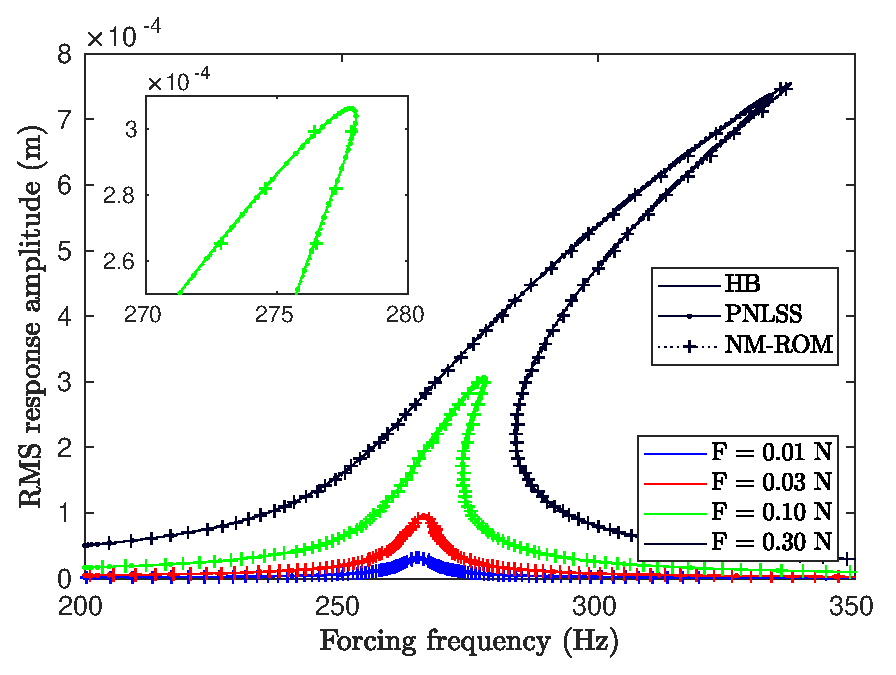
\includegraphics[width=\linewidth]{{{../../benchmark1/extabs_fig/b1_fresp_comp_A0.50_nx23}}}
    \end{subfigure}%
    \begin{subfigure}{0.25\linewidth}
      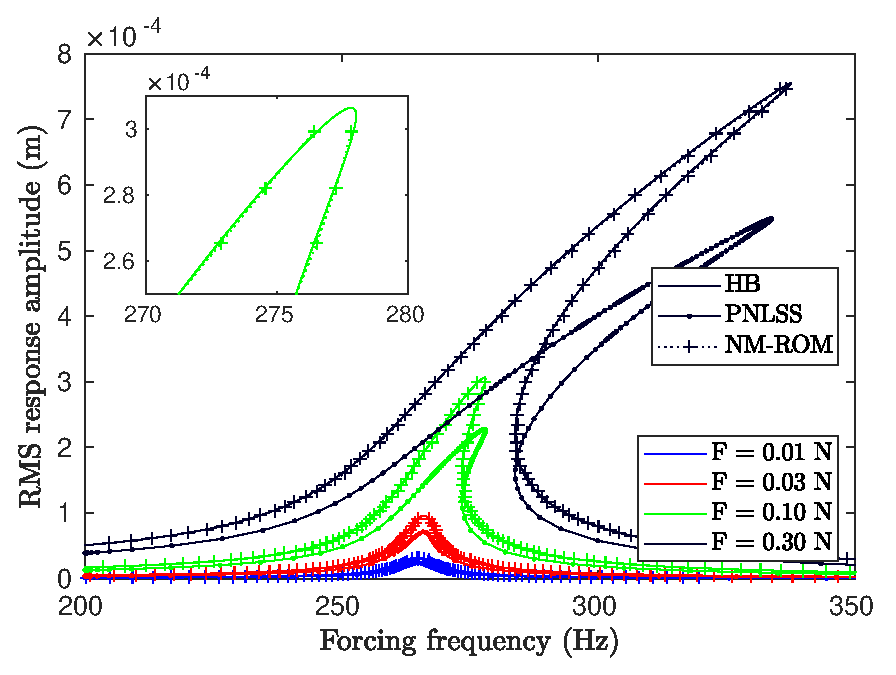
\includegraphics[width=\linewidth]{{{../../benchmark1/extabs_fig/b1_fresp_comp_A0.75_nx23}}}
    \end{subfigure}

    \begin{subfigure}{0.25\linewidth}
      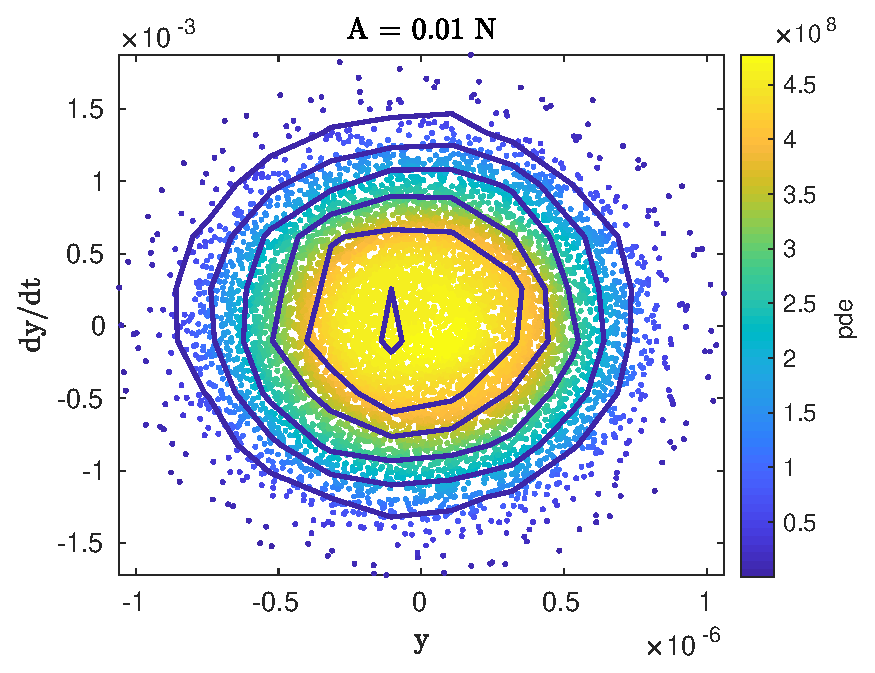
\includegraphics[width=\linewidth]{{{../../benchmark1/extabs_fig/b1_tdata_kern_A0.01}}}
      \caption{A=0.01 N}
    \end{subfigure}%
    \begin{subfigure}{0.25\linewidth}
      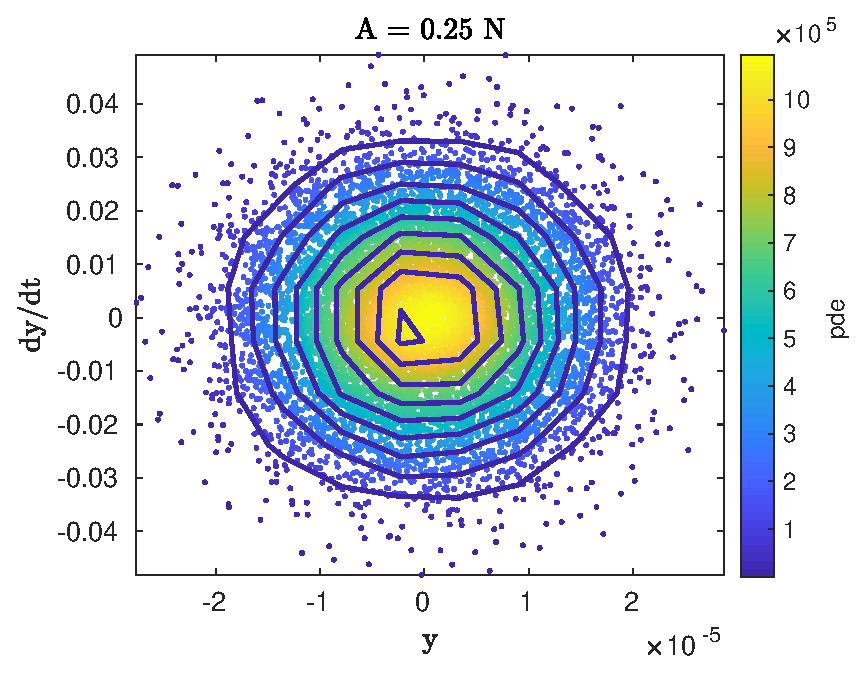
\includegraphics[width=\linewidth]{{{../../benchmark1/extabs_fig/b1_tdata_kern_A0.25}}}
      \caption{A=0.25 N}
    \end{subfigure}%
    \begin{subfigure}{0.25\linewidth}
      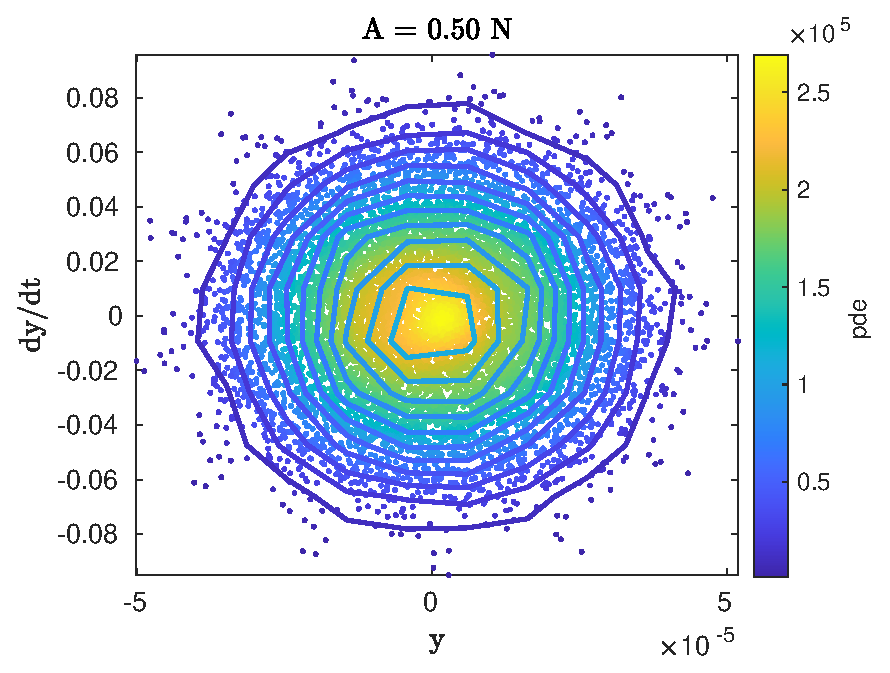
\includegraphics[width=\linewidth]{{{../../benchmark1/extabs_fig/b1_tdata_kern_A0.50}}}
      \caption{A=0.50 N}
    \end{subfigure}%
    \begin{subfigure}{0.25\linewidth}
      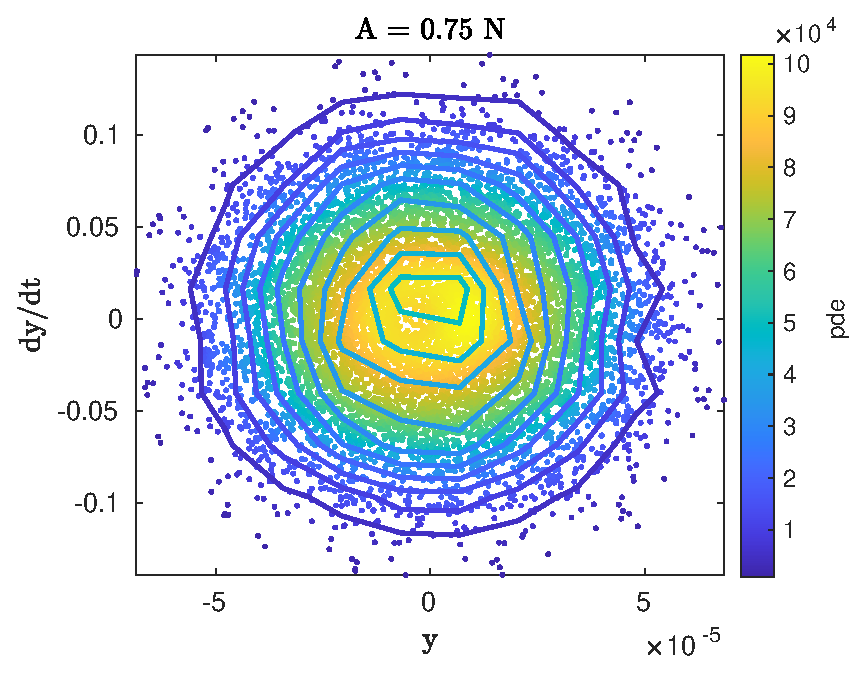
\includegraphics[width=\linewidth]{{{../../benchmark1/extabs_fig/b1_tdata_kern_A0.75}}}
      \caption{A=0.75 N}
    \end{subfigure}
  \end{figure}
\end{frame}

\section{Benchmark 4}
\label{sec:benchmark-4}

\begin{frame}
  \frametitle{Progress on Benchmark 4 (Beam with friction)}
  \framesubtitle{Overview}
  \begin{itemize}
  \item Conducted PNLSS with different amplitude levels (as before)
  \item Constructed frequency response with PNLSS model (!)
    \begin{itemize}
    \item This was found to be extremely sensitive to the continuation
      parameters
    \item In order to get decent figures I had to use the previous
      version of nlvib (2017), which had a slightly different
      terminator condition
    \end{itemize}
  \item Synthesized frequency response from simulated PLL experiments
    from Eve (without shaker)
    \begin{itemize}
    \item She's given me the codes for doing it with the shaker, I
      just need to add the shaker model for the transient simulations
    \item Should be good to go soon
    \end{itemize}
  \end{itemize}
  \textbf{To Do:}
  \begin{itemize}
  \item \alert{Employ PLL data for PNLSS identification}    
  \item Identify approaches to reduce amplitude dependence
    \begin{itemize}
    \item Currently looking into triangle-modulated multi-sines
      (sawtooths were leaking too much)
    \end{itemize}
  \end{itemize}
\end{frame}

\begin{frame}[allowframebreaks]
  \frametitle{Progress on Benchmark 4 (Beam with friction)}
  \framesubtitle{PNLSS training (vanilla version)}
  \vspace{-0.5cm}
  \begin{figure}[!h]
    \centering
    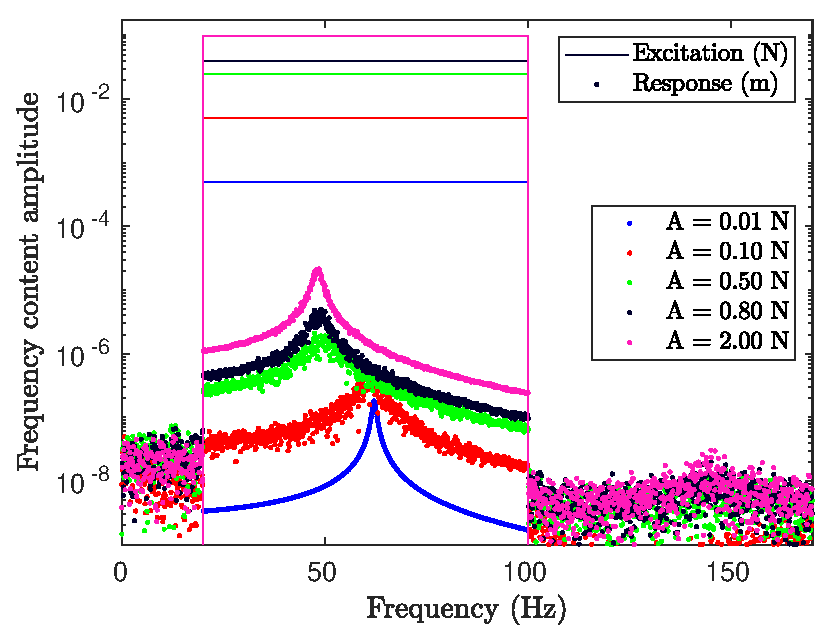
\includegraphics[width=0.5\linewidth]{../../benchmark4/extabs_fig/b4_tdata_freqcont}
    \caption{Frequency content of different multi-sine
      responses showing stick-slip.}
  \end{figure}
  
  \begin{figure}[!h]
    \centering
    \begin{subfigure}{0.2\linewidth}
      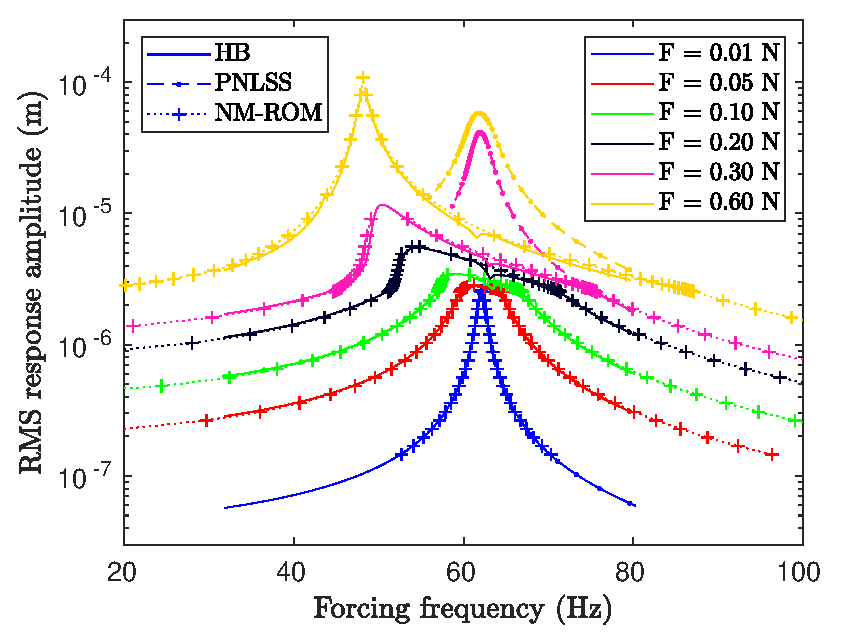
\includegraphics[width=\linewidth]{../../benchmark4/extabs_fig/b4_fresp_comp_famp001_nx23}
    \end{subfigure}%
    \begin{subfigure}{0.2\linewidth}
      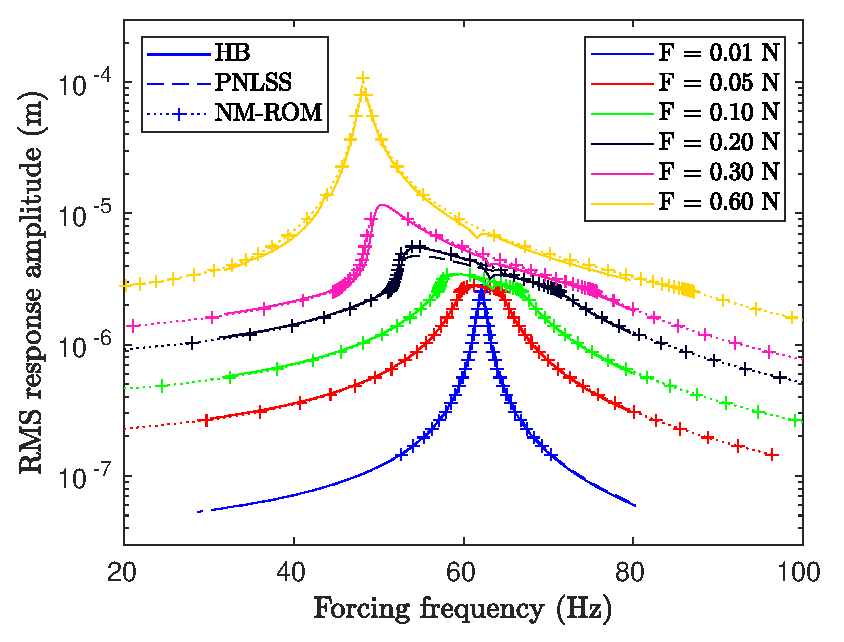
\includegraphics[width=\linewidth]{../../benchmark4/extabs_fig/b4_fresp_comp_famp01_nx23}
    \end{subfigure}%
    \begin{subfigure}{0.2\linewidth}
      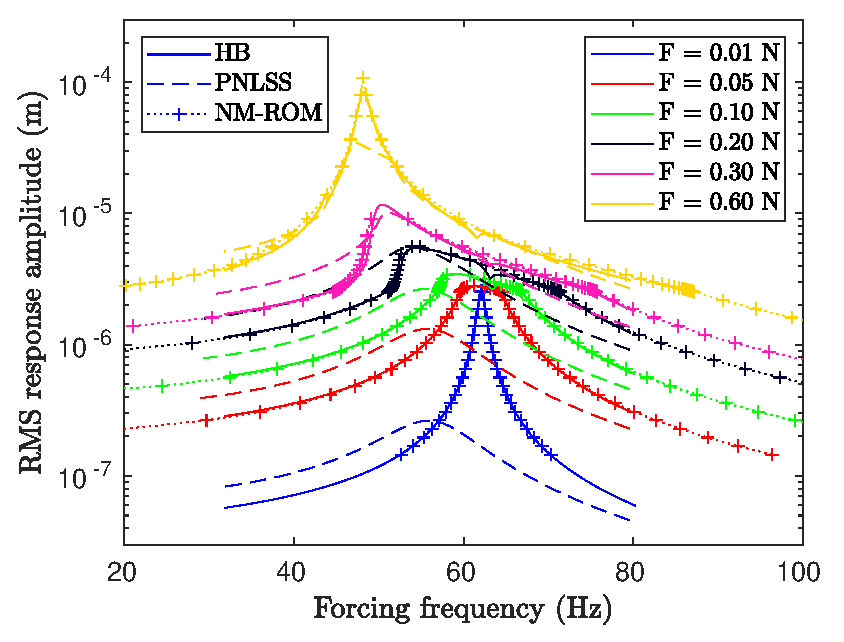
\includegraphics[width=\linewidth]{../../benchmark4/extabs_fig/b4_fresp_comp_famp05_nx23}
    \end{subfigure}%
    \begin{subfigure}{0.2\linewidth}
      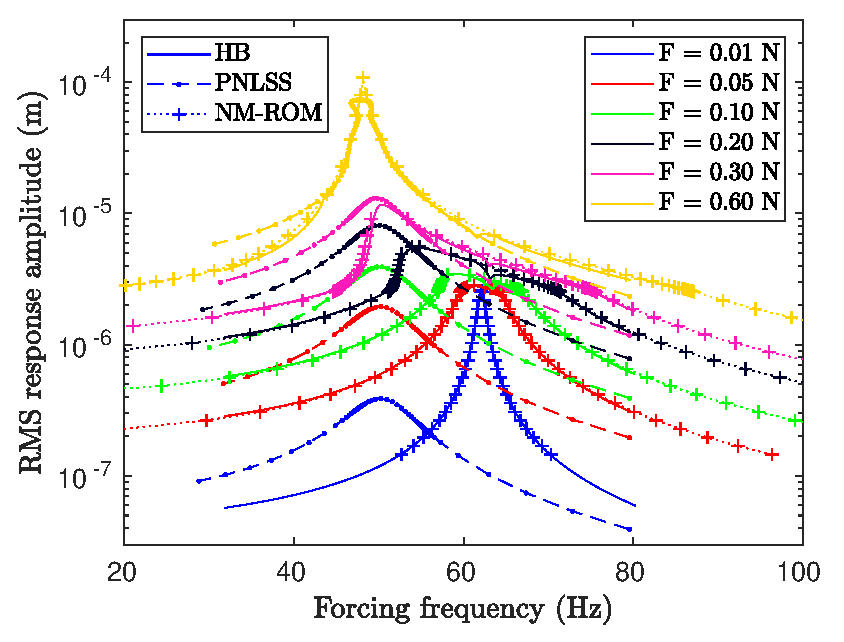
\includegraphics[width=\linewidth]{../../benchmark4/extabs_fig/b4_fresp_comp_famp08_nx23}
    \end{subfigure}%
    \begin{subfigure}{0.2\linewidth}
      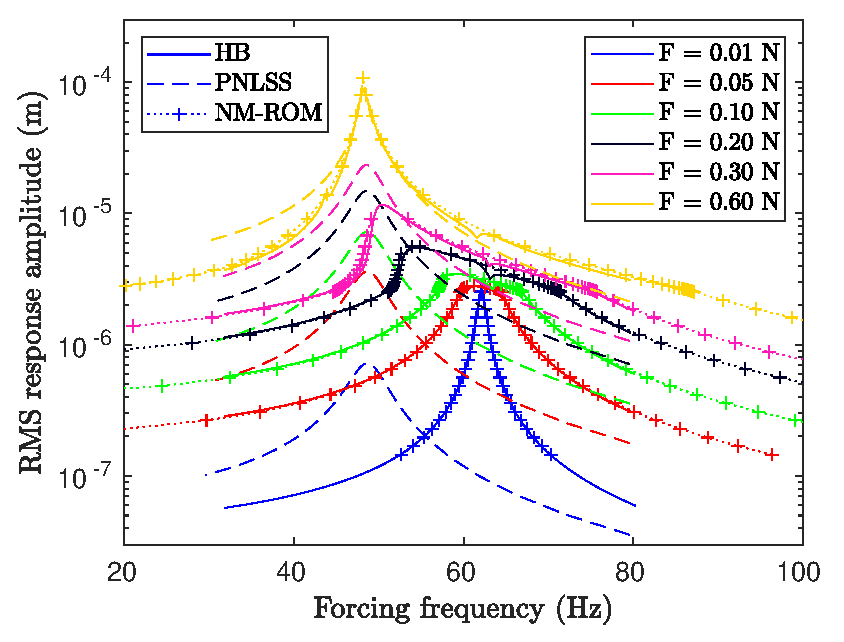
\includegraphics[width=\linewidth]{../../benchmark4/extabs_fig/b4_fresp_comp_famp20_nx23}
    \end{subfigure}%
    
    \begin{subfigure}{0.2\linewidth}
      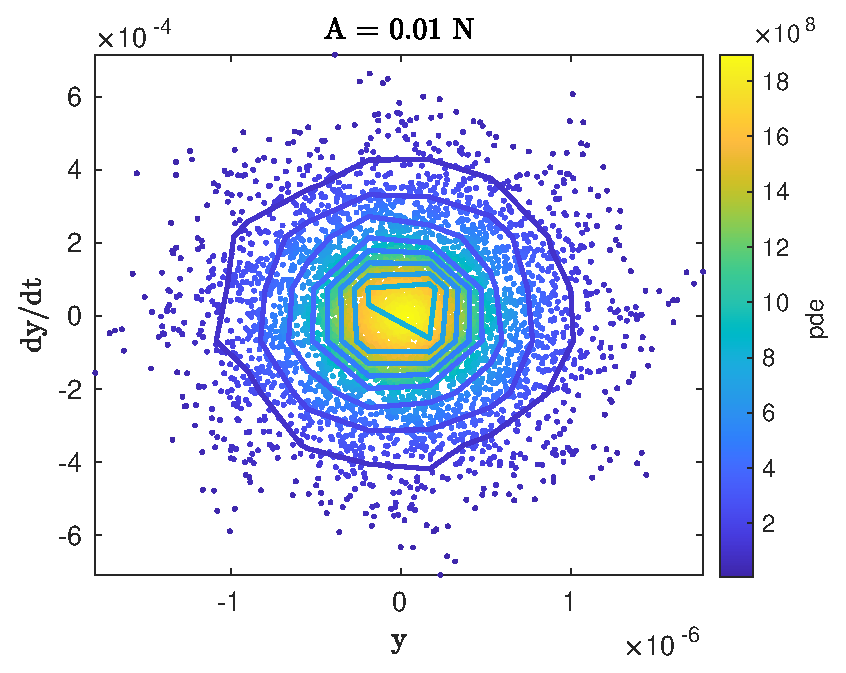
\includegraphics[width=\linewidth]{../../benchmark4/extabs_fig/b4_tdata_kern_famp001}
      \caption{A = 0.001 N}
    \end{subfigure}%
    \begin{subfigure}{0.2\linewidth}
      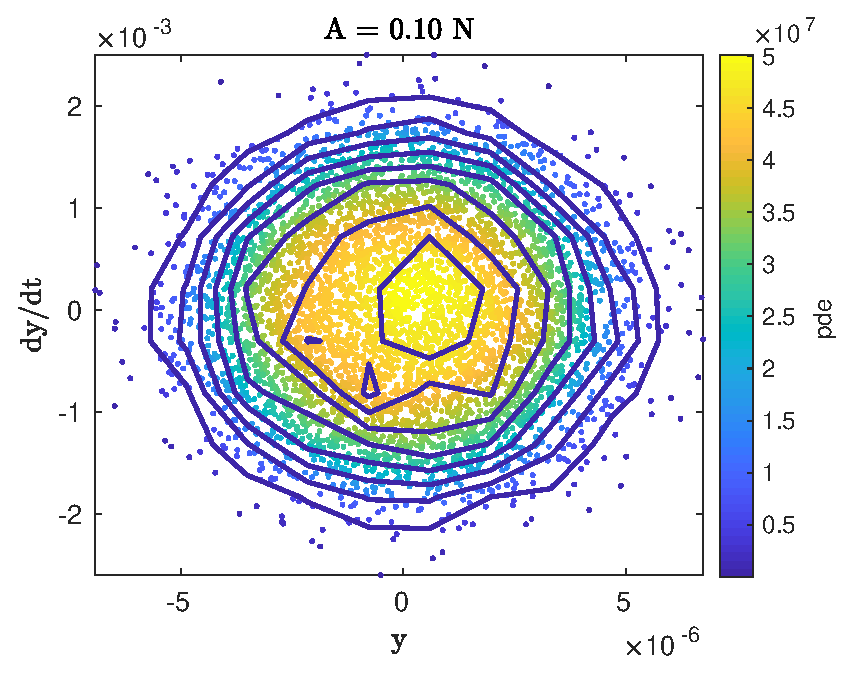
\includegraphics[width=\linewidth]{../../benchmark4/extabs_fig/b4_tdata_kern_famp01}
      \caption{A = 0.01 N}
    \end{subfigure}%
    \begin{subfigure}{0.2\linewidth}
      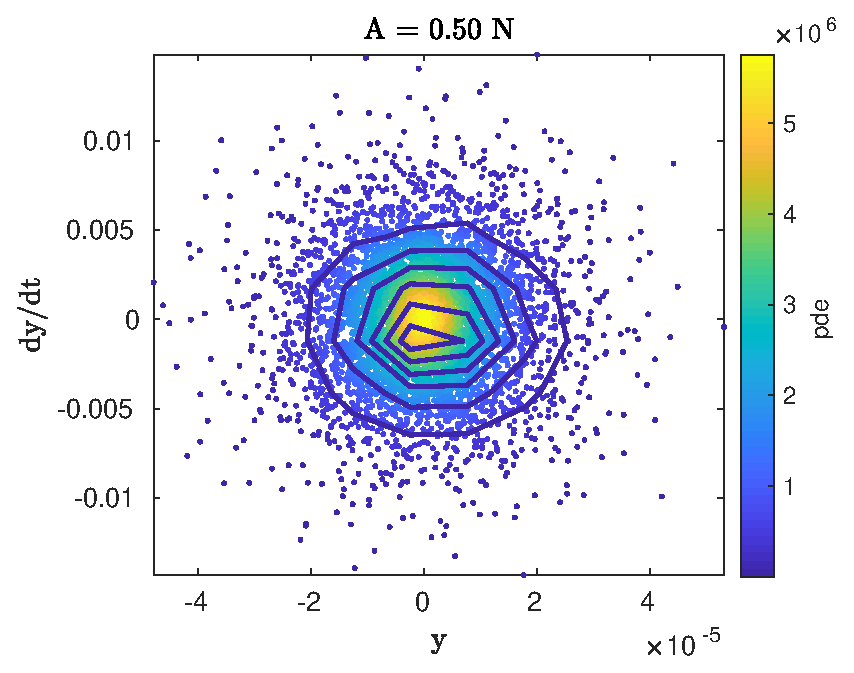
\includegraphics[width=\linewidth]{../../benchmark4/extabs_fig/b4_tdata_kern_famp05}
      \caption{A = 0.05 N}
    \end{subfigure}%
    \begin{subfigure}{0.2\linewidth}
      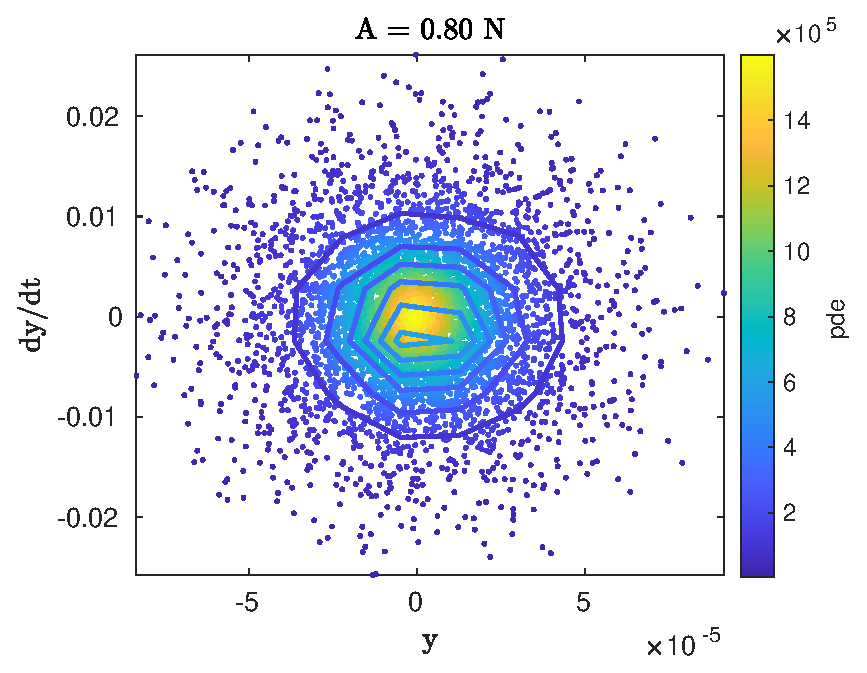
\includegraphics[width=\linewidth]{../../benchmark4/extabs_fig/b4_tdata_kern_famp08}
      \caption{A = 0.08 N}
    \end{subfigure}%
    \begin{subfigure}{0.2\linewidth}
      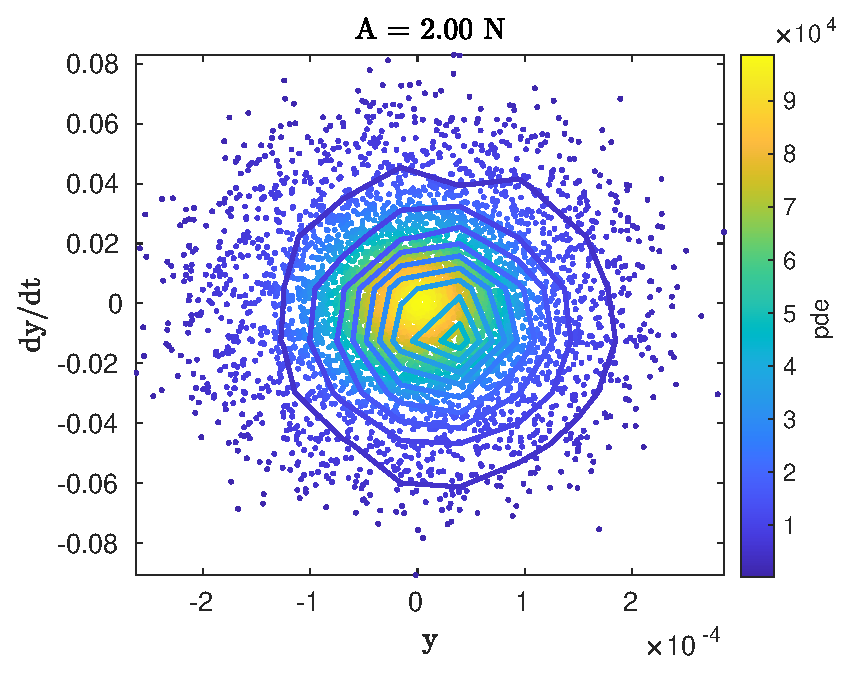
\includegraphics[width=\linewidth]{../../benchmark4/extabs_fig/b4_tdata_kern_famp20}
      \caption{A = 0.20 N}
    \end{subfigure}%    
  \end{figure}
\end{frame}

\begin{frame}
  \frametitle{Progress on Benchmark 4 (Beam with friction)}
  \framesubtitle{Emloying PLL Data for PNLSS Identification}
  \textbf{Approach so far:}
  \begin{itemize}
  \item Use low amplitude multi-sine data for BLA initialization
  \item Use PLL data for PNLSS identification
  \end{itemize}
  \textbf{Problem:}
  \begin{itemize}
  \item Unable to get optimization to reduce error sufficiently
    well. Best I could get:
    \begin{figure}[!h]
      \centering
      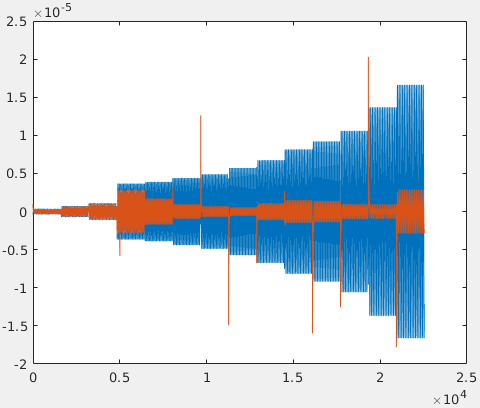
\includegraphics[width=0.3\linewidth]{FIGS/pnlss_pll}
    \end{figure}
  \end{itemize}
\end{frame}

\begin{frame}[allowframebreaks]
  \frametitle{Progress on Benchmark 4 (Beam with friction)}
  \framesubtitle{Circumventing Amplitude Dependence}
  \vspace{-0.8cm}
  \begin{figure}
    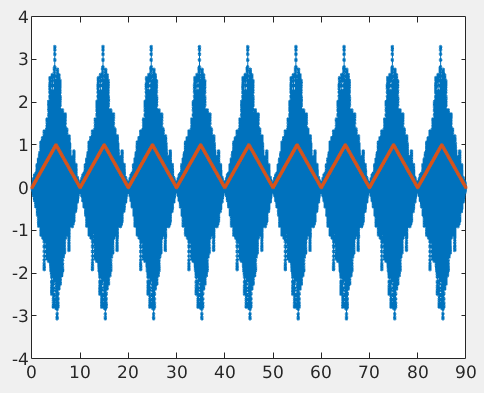
\includegraphics[width=0.5\linewidth]{FIGS/triangle_mod}
    \caption{Triangle-modulated multi-sine}
  \end{figure}
  
  \begin{figure}
    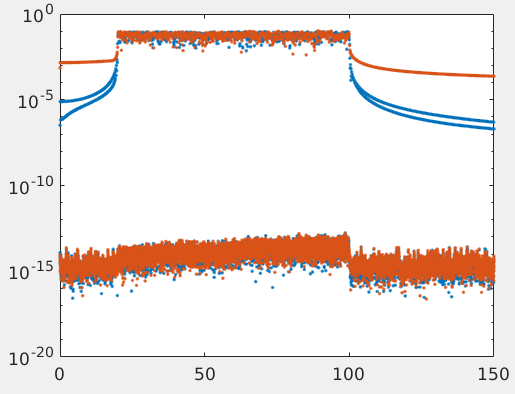
\includegraphics[width=0.5\linewidth]{FIGS/leakage_comp}
    \caption{Leakage: triangle vs sawtooth}
  \end{figure}%
\end{frame}

\section{Outlook}
\label{sec:outlook}

\begin{frame}
  \frametitle{Outlook}
  At this point, I think it makes sense to determine the primary focus
  for each benchmark. I have made the following list based on what
  makes sense to me and would like to discuss on it:
  \begin{description}
  \item[Benchmark 1] (Geometrically non-linear beam modeled as
    \underline{SDOF Duffing oscillator})\\
    The focus could be capturing the stiffening non-linearity.
  \item[Benchmark 2] (MDOF model with cubic non-linearities)\\
    The focus could be capturing \underline{2/3 modes simultaneously}. PNLSS
    could be trained using multisines with bands limited around
    multiple modes at the same time (we already have initial results
    from the summer).
  \item[Benchmark 3] (MDOF model with softening-stiffening
    non-linearity)\\
    The focus could be capturing the softening-stiffening effect for
    \underline{mode 1 alone}.
  \item[Benchmark 4] (E-B Beam with frictional node)\\
    The focus could be capturing the dampening-softening effect for
    \underline{mode 1 alone}.
  \item[Benchmark 5] (E-B Beam with unilateral contacting node)\\
    The focus could be capturing the contacting-stiffening effect for
    \underline{mode 1 alone}.
  \end{description}
\end{frame}
\end{document}
%%% Local Variables:
%%% mode: latex
%%% TeX-master: t
%%% End:
